\cleardoublepage % memastikan bab baru dimulai di halaman ganjil (kanan)
\chapter{STUDI LITERATUR}
\label{chap:studi-literatur}

\section{Pembelajaran Algoritma dan Struktur Data (ASD)}

Bagian ini membahas landasan teoritis mengenai Algoritma dan Struktur Data (ASD) sebagai domain materi yang menjadi fokus aplikasi yang dikembangkan. Kajian mencakup konsep dasar ASD serta karakteristik kesulitan yang umum dialami mahasiswa dalam mempelajarinya.

\subsection{Konsep Dasar Algoritma dan Struktur Data}

Algoritma dan Struktur Data (ASD) merupakan mata kuliah fundamental dalam ilmu komputer karena berfokus pada cara menyusun, menyimpan, dan mengelola data secara efisien. Algoritma dipahami sebagai serangkaian langkah terstruktur untuk menyelesaikan suatu permasalahan, sedangkan struktur data berkaitan dengan cara merepresentasikan dan mengorganisasikan data dalam memori komputer \cite{Cormen2009CLRS}. Pemahaman terhadap ASD sangat penting karena konsep-konsep ini menjadi dasar bagi pemrograman, optimasi performa program, analisis kompleksitas waktu dan ruang, manajemen memori, hingga perancangan sistem berskala besar \cite{Goodrich1998DSAJava}.

Materi ASD umumnya mencakup struktur dasar seperti \textit{array}, \textit{linked list}, \textit{stack}, \textit{queue}, \textit{heap}, \textit{tree}, \textit{graph}, serta algoritma pencarian (\textit{searching}) dan pengurutan (\textit{sorting}). Penguasaan materi ini tidak hanya membutuhkan kemampuan memahami definisi dan contoh, tetapi juga keterampilan menalar alur eksekusi program, memahami perubahan data secara dinamis, dan menganalisis performa algoritma di berbagai kondisi masukan. Tantangan ini sering menjadi penyebab kesulitan belajar mahasiswa dalam memahami konsep ASD, sebagaimana ditunjukkan dalam studi literatur mengenai hambatan umum pembelajaran struktur data dan algoritma \cite{Mtaho2024}.

\subsection{Kesulitan Mahasiswa dalam Mempelajari ASD}

Berbagai penelitian menunjukkan bahwa mahasiswa sering mengalami kesulitan dalam mempelajari Algoritma dan Struktur Data (ASD) karena sifat materinya yang abstrak, dinamis, dan multidimensional. Berdasarkan temuan dari \textit{systematic literature review} yang dilakukan oleh Mtaho dan Mselle \cite{Mtaho2024}, kesulitan terbesar mahasiswa berasal dari beberapa faktor utama, yaitu:

\begin{enumerate}
    \item Abstraksi konsep yang tinggi, sehingga sulit untuk divisualisasikan. Contohnya adalah konsep \textit{pointer}, \textit{node}, atau relasi antar-\textit{node} pada struktur \textit{tree} dan \textit{graph} yang tidak terlihat secara langsung dalam eksekusi program.

    \item Perubahan struktur yang bersifat dinamis, seperti pemutakhiran referensi pada \textit{linked list} atau proses rotasi pada \textit{binary tree}. Perubahan ini menuntut kemampuan visualisasi mental dan penalaran yang kuat untuk memahami bagaimana data bergerak dan dimodifikasi.

    \item Beban kognitif yang tinggi, karena pembelajaran ASD mengharuskan mahasiswa memahami representasi struktur data, logika algoritma, serta implementasi kode secara bersamaan. Tuntutan ini sering membuat mahasiswa kewalahan ketika mencoba menghubungkan teori dengan implementasi.

    \item Miskonsepsi pada konsep dasar, seperti salah memahami operasi \textit{insert} atau \textit{delete}, cara kerja \textit{pointer}, atau alur eksekusi algoritma. Miskonsepsi tersebut dapat menghambat pemahaman materi lanjutan dan berdampak pada kemampuan pemecahan masalah.
\end{enumerate}


% LLM
\section{Large Language Model (LLM)}

Bagian ini menguraikan landasan teoritis mengenai \textit{Large Language Model} (LLM) yang digunakan sebagai komponen inti dalam aplikasi. Kajian meliputi konsep dasar dan mekanisme kerja LLM serta teknik \textit{prompt engineering} yang digunakan untuk mengarahkan keluaran model agar relevan dan konsisten dengan kurikulum ASD.

\subsection{Konsep Dasar dan Mekanisme LLM}

\textit{Large Language Model} (LLM) merupakan model kecerdasan buatan berskala besar yang dirancang untuk mempelajari struktur bahasa dan memprediksi token berikutnya berdasarkan konteks masukan. Model ini dilatih menggunakan kumpulan data berukuran sangat besar (miliaran token) dan parameter berskala tinggi sehingga mampu melakukan berbagai tugas pemrosesan bahasa secara generatif, seperti menjawab pertanyaan, merangkum teks, menjelaskan konsep, hingga menghasilkan kode program.

Arsitektur utama yang menjadi fondasi LLM modern adalah Transformer \cite{Vaswani2017AttentionIsAllYouNeed}, yang mengandalkan mekanisme \textit{self-attention} untuk memahami hubungan antar-token secara paralel dan efisien. Transformer terdiri dari dua komponen utama, yaitu \textit{encoder} dan \textit{decoder}, tetapi mayoritas LLM generatif saat ini (seperti GPT dan model berbasis \textit{decoder-only} lainnya) hanya menggunakan blok \textit{decoder}. Setiap \textit{decoder layer} terdiri dari beberapa komponen inti yang memproses \textit{input} secara bertahap.

\begin{figure}[H]
    \centering
    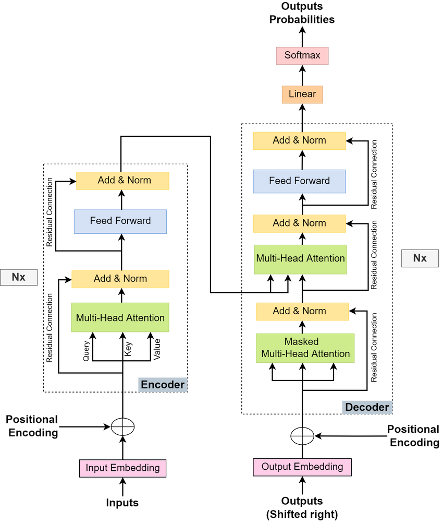
\includegraphics[width=0.75\textwidth]{images/transformer-architecture.png}
    \caption{Arsitektur dasar Transformer}
    \label{fig:transformer}
\end{figure}

Secara umum, proses kerja LLM dapat dijelaskan melalui beberapa tahapan berikut:

\begin{enumerate}
    \item \textit{Tokenization}: masukan teks diubah menjadi serangkaian token menggunakan metode seperti BPE (\textit{Byte Pair Encoding}) atau \textit{SentencePiece}. Token inilah yang diproses oleh model.

    \item \textit{Input Embedding}: setiap token direpresentasikan sebagai vektor berdimensi tinggi (misalnya 512--4096 dimensi), sehingga dapat diproses secara numerik oleh jaringan saraf.

    \item \textit{Positional Encoding}: karena Transformer tidak memiliki konsep urutan secara bawaan, informasi posisi ditambahkan menggunakan \textit{positional encoding} sinusoidal atau embedding terlatih lainnya.

    \item \textit{Multi-Head Self-Attention}: setiap token menghitung relevansinya terhadap token lain menggunakan tiga vektor utama: Query (Q), Key (K), dan Value (V). Mekanisme perhatian dihitung menggunakan rumus:

    \[
        \text{Attention}(Q, K, V) = \text{softmax}\left( \frac{QK^{T}}{\sqrt{d_k}} \right) V
    \]

    Mekanisme ini memungkinkan model mengidentifikasi konteks penting, dependensi jarak jauh, serta memahami relasi antar-token secara paralel melalui beberapa \textit{attention heads}.

    \item \textit{Feed-Forward Network (FFN)}: setiap token melewati jaringan \textit{feed-forward} dua lapis dengan aktivasi non-linear. Komponen ini memperluas kapasitas representasi sehingga model mampu melakukan transformasi dan \textit{reasoning} yang lebih kompleks.

    \item \textit{Output Softmax Layer}: pada tahap akhir, LLM memprediksi token berikutnya dengan memilih probabilitas tertinggi dari distribusi keluaran. Proses ini dilakukan secara autoregresif hingga seluruh respons terbentuk.
\end{enumerate}

Dengan kombinasi arsitektur Transformer dan pelatihan berskala besar, LLM memiliki kemampuan memahami konteks secara mendalam, menghasilkan teks yang koheren, serta menyesuaikan gaya bahasa sesuai kebutuhan pengguna.


\subsection{\textit{Prompt Engineering}}

\textit{Prompt} merupakan masukan teks yang diberikan pengguna untuk memandu model kecerdasan buatan, seperti LLM, dalam menghasilkan keluaran yang relevan dan sesuai tujuan. Dalam \textit{Prompt Engineering}, proses ini melibatkan perancangan \textit{prompt} yang efektif melalui pemilihan instruksi, konteks, contoh, serta batasan tertentu agar model dapat memberikan respons yang lebih akurat, terarah, dan konsisten. Teknik ini menjadi semakin penting karena performa LLM sangat bergantung pada cara instruksi dirumuskan dan seberapa jelas konteks yang diberikan \cite{Minaee2025PromptEngineering, White2023PromptPatternCatalog}.

Berbagai strategi \textit{prompt engineering} telah dikembangkan untuk meningkatkan performa LLM dalam menyelesaikan tugas-tugas kompleks. Beberapa teknik utama yang umum digunakan adalah sebagai berikut:

\begin{enumerate}
    \item \textit{Zero-Shot Prompting}: model diminta menyelesaikan tugas tanpa contoh sebelumnya, hanya berdasarkan instruksi.

    \item \textit{Few-Shot Prompting}: pengguna memberikan beberapa contoh masukan–keluaran untuk membimbing model menghasilkan respons yang serupa.

    \item \textit{Chain of Thought (CoT)}: instruksi meminta model menjelaskan proses berpikir secara bertahap, sehingga meningkatkan akurasi pada tugas penalaran.

    \item \textit{Tree of Thought (ToT)}: model mengeksplorasi beberapa jalur penalaran, mengevaluasi setiap opsi, kemudian memilih solusi terbaik.

    \item \textit{Self-Consistency}: model menghasilkan beberapa jalur penalaran yang kemudian digabungkan untuk memperoleh jawaban paling konsisten.

    \item \textit{Reflection Prompting}: setelah memberikan jawaban, model diminta melakukan evaluasi diri dan memperbaiki respons sebelumnya.

    \item \textit{Expert Prompting}: model diarahkan untuk bertindak sebagai seorang pakar dalam domain tertentu agar kualitas penjelasan lebih mendalam dan terstruktur.

    \item \textit{Rails / Guardrails}: pemberian batasan dan instruksi khusus agar model tetap fokus pada topik yang relevan serta mengurangi risiko \textit{hallucination}.

    \item \textit{Automatic Prompt Engineering (APE)}: menggunakan LLM untuk menghasilkan, menguji, dan memilih \textit{prompt} terbaik secara otomatis.
\end{enumerate}

Teknik-teknik tersebut digunakan untuk meningkatkan kontrol pengguna terhadap keluaran model, mengurangi risiko bias atau kesalahan, serta meningkatkan kualitas penjelasan dan kemampuan penalaran LLM dalam berbagai konteks pembelajaran maupun aplikasi praktis.

\subsection{Pemanfaatan LLM dalam Proses Pembelajaran}

Berbagai penelitian menunjukkan bahwa LLM semakin banyak dimanfaatkan sebagai sarana untuk memudahkan proses pembelajaran, baik sebagai tutor personal, penyedia umpan balik otomatis, maupun pendamping belajar mandiri. Kasneci dkk. \cite{Kasneci2023} mengidentifikasi bahwa LLM berpotensi meningkatkan personalisasi pembelajaran melalui kemampuannya menyesuaikan penjelasan dengan tingkat pemahaman pengguna, menyediakan umpan balik yang instan, serta mendukung akses belajar yang fleksibel tanpa batasan waktu dan tempat, sekaligus menyoroti tantangan terkait akurasi konten dan potensi ketergantungan berlebihan pada teknologi.

Dalam konteks pendidikan pemrograman, Leinonen dkk. \cite{Leinonen2023} menunjukkan bahwa LLM dapat digunakan untuk menerjemahkan pesan kesalahan pemrograman yang teknis menjadi penjelasan yang lebih mudah dipahami pemula, sehingga mempercepat proses \textit{debugging} dan mengurangi frustrasi belajar. Sejalan dengan itu, Jacobs dan Jaschke \cite{Jacobs2024LLMFeedbackProgramming} mengevaluasi penerapan LLM untuk menghasilkan umpan balik otomatis pada tugas pemrograman dan menemukan bahwa umpan balik yang dihasilkan cukup relevan serta membantu mahasiswa memahami letak kesalahan mereka secara mandiri.

Pemanfaatan LLM sebagai tutor personal juga dikaji oleh Vanzo dkk. \cite{Vanzo2024GPT4HomeworkTutor}, yang menemukan bahwa penggunaan GPT-4 sebagai pendamping mengerjakan tugas mampu meningkatkan keterlibatan dan capaian belajar mahasiswa dibandingkan metode belajar konvensional. Namun, tinjauan sistematis oleh Raihan dkk. \cite{Raihan2024} terhadap penerapan LLM dalam pendidikan ilmu komputer menegaskan bahwa manfaat tersebut hanya dapat dicapai secara konsisten apabila interaksi LLM diarahkan melalui mekanisme yang terstruktur, mengingat penggunaan LLM secara bebas berisiko menghasilkan penjelasan yang tidak konsisten atau menyimpang dari kurikulum.

Secara keseluruhan, pemanfaatan LLM dalam pembelajaran menunjukkan pergeseran peran teknologi dari sekadar alat pencarian informasi menjadi teman belajar interaktif yang mampu menjelaskan, mengoreksi, dan membimbing pengguna secara kontekstual. Temuan-temuan ini menjadi landasan bagi penelitian ini untuk mengembangkan Teman Belajar ASD sebagai aplikasi yang memanfaatkan LLM secara terarah guna mendukung proses belajar mandiri mahasiswa.

% Evaluasi
\section{Evaluasi}

Bagian ini membahas metode evaluasi yang digunakan untuk menilai kualitas dan kegunaan aplikasi yang dikembangkan. Kajian mencakup pendekatan \textit{black box testing} untuk verifikasi fungsionalitas sistem serta \textit{System Usability Scale} (SUS) sebagai instrumen pengukuran kegunaan.

\subsection{\textit{Black Box Testing}}

\textit{Black Box Testing} merupakan metode pengujian perangkat lunak yang berfokus pada evaluasi fungsi dan perilaku sistem dari sisi eksternal tanpa melihat struktur internal atau kode program. Pengujian dilakukan dengan memberikan berbagai \textit{input} dan memeriksa apakah \textit{output} yang dihasilkan telah sesuai dengan spesifikasi yang ditentukan \cite{Pressman2015SWE}.

Salah satu teknik \textit{Black Box Testing} yang banyak digunakan adalah \textit{Equivalence Partitioning}, yaitu pendekatan yang membagi domain \textit{input} ke dalam beberapa kelas ekivalen sehingga hanya satu nilai per kelas yang perlu diuji. Setiap nilai dalam kelas tersebut dianggap mewakili perilaku sistem untuk seluruh anggota kelas. Teknik ini membantu mengurangi jumlah \textit{test case} tanpa menurunkan efektivitas pengujian karena setiap partisi dirancang untuk menangkap potensi kesalahan berdasarkan kelompok \textit{input} yang memiliki karakteristik serupa \cite{Pressman2015SWE}.

Selain itu, pendekatan ini memperkuat efisiensi proses pengujian karena dapat meminimalkan redundansi dan meningkatkan cakupan pengujian. Konsep \textit{Equivalence Partitioning} juga didukung oleh pendekatan lain dalam pengujian perangkat lunak yang menekankan pentingnya representasi kelas nilai uji dalam mendeteksi kesalahan secara sistematis \cite{Myers2011ArtOfSoftwareTesting}. Dengan demikian, teknik ini menjadi salah satu metode yang efektif untuk memastikan bahwa fungsi utama perangkat lunak bekerja sesuai dengan spesifikasi yang telah ditetapkan.


\section{Penelitian Terdahulu}

Bagian ini mengulas penelitian-penelitian terdahulu yang relevan dengan topik pengembangan aplikasi pembelajaran ASD berbasis LLM. Kajian terhadap penelitian terdahulu dilakukan untuk mengidentifikasi pendekatan yang telah digunakan, hasil yang diperoleh, serta celah penelitian yang menjadi landasan pengembangan sistem dalam Tugas Akhir ini.

\subsection{\textit{Utilizing ChatGPT in a Data Structures and Algorithms Course: A Teaching Assistant's Perspective}}

Pemanfaatan ChatGPT sebagai alat bantu \textit{Teaching Assistant} (TA) dalam mata kuliah \textit{Data Structures and Algorithms} (DSA) terbukti efektif dalam meningkatkan kualitas pembelajaran. Studi oleh Jamie et al. \cite{Jamie2024ChatGPTDSA} menunjukkan bahwa penggunaan LLM seperti ChatGPT-4o dan ChatGPT-o1 dapat membantu mahasiswa memahami konsep algoritmik kompleks melalui penjelasan terstruktur, pembuatan contoh, dan penyediaan latihan berbasis \textit{structured prompts}. Dalam pendekatan ini, keluaran LLM tetap diverifikasi oleh TA untuk menjaga akurasi dan kesesuaian konten.

Hasil eksperimen terkontrol membandingkan dua kelas---kelas dengan instruksi tradisional dan kelas dengan pendekatan hibrida TA dengan ChatGPT. Kelompok hibrida menunjukkan peningkatan signifikan dengan selisih rata-rata 16{,}50 poin lebih tinggi pada latihan, kuis, dan ujian. Model AI membantu menjelaskan konsep sulit seperti rekursi, \textit{graph traversal}, serta \textit{dynamic programming}, sembari menyajikan keluaran yang lebih terarah berkat \textit{prompt} yang sistematis.

Namun, penelitian tersebut juga mencatat keterbatasan ChatGPT, seperti ketidakmampuan menghasilkan visualisasi struktur data dan potensi kesalahan pada masalah yang memerlukan kreativitas tinggi. Dengan demikian, peran TA tetap penting untuk memvalidasi keluaran model. Studi ini menegaskan bahwa integrasi LLM tidak menggantikan peran manusia, melainkan memperkuat efektivitas pengajaran melalui kolaborasi manusia dan AI yang terstruktur.


\subsection{\textit{Evaluating the Effectiveness of Large Language Models in Solving Simple Programming Tasks: A User-Centered Study}}

Penelitian oleh Deng \cite{Deng2025LLMProgrammingTasks} mengevaluasi efektivitas tiga gaya interaksi ChatGPT-4o, \textit{Passive}, \textit{Proactive}, dan \textit{Collaborative}, dalam membantu pengguna menyelesaikan tugas pemrograman sederhana. Pada mode \textit{Passive}, model hanya merespons permintaan. Pada mode \textit{Proactive}, model memberikan saran tambahan, sedangkan mode \textit{Collaborative} memungkinkan diskusi dua arah yang lebih intens.

Sebanyak lima belas siswa sekolah menengah diminta menyelesaikan tiga soal pemrograman di setiap mode interaksi. Hasil eksperimen menunjukkan bahwa mode \textit{Collaborative} menghasilkan waktu penyelesaian tercepat, yaitu rata-rata 2{,}63 menit per soal, dibandingkan mode \textit{Passive} yang membutuhkan rata-rata 3{,}60 menit. Hal ini menunjukkan bahwa kualitas interaksi berperan penting dalam efektivitas penggunaan LLM.

Selain peningkatan performa, peserta juga melaporkan tingkat kepuasan dan persepsi kebermanfaatan yang lebih tinggi pada mode \textit{Collaborative}. Temuan ini menegaskan bahwa interaksi yang bersifat dialogis membantu pengguna memahami langkah penyelesaian masalah dengan lebih baik.


\subsection{\textit{Leveraging Algorithm Instruction with AI Chatbots: A Detailed Exploration of Their Impact on Students' Computational Thinking}}

Penggunaan \textit{AI-based chatbots} sebagai pendukung pembelajaran algoritma turut dievaluasi oleh Zaus et al. \cite{Zaus2025AlgorithmInstructionChatbots}. Melalui pendekatan \textit{quasi-experimental}, penelitian ini membandingkan kelompok mahasiswa yang belajar dengan bantuan \textit{chatbot} dan kelompok yang menggunakan metode pembelajaran konvensional.

Hasil \textit{pre-test} dan \textit{post-test} menunjukkan peningkatan signifikan pada pemahaman konsep algoritma dan keterampilan \textit{computational thinking} dalam kelompok yang menggunakan \textit{chatbot}. Hal ini terjadi karena \textit{chatbot} menyediakan penjelasan langkah demi langkah, umpan balik otomatis, serta dukungan koreksi kesalahan yang membuat proses belajar lebih interaktif dan mudah diikuti.

Penelitian ini juga menemukan bahwa \textit{chatbot} dapat berfungsi sebagai bentuk \textit{scaffolding}, membantu mahasiswa mengatasi miskonsepsi pada materi yang kompleks, serta menyesuaikan tingkat kesulitan penyampaian materi berdasarkan respons pengguna. Dengan demikian, pengalaman belajar menjadi lebih personal dan adaptif.
